\chapter{Preliminares}

Para el análisis del módelo presa-depredador tipo Leslie-Gower con respuesta funcional sigmoidea que se lleva acabo en el presente trabajo, requerimos de ciertos conceptos fundamentales, los cuales se abarcan en la presente sección, esto, con el objetivo de lograr una mejor compresión de todo lo que se presenta posteriormente.

\section*{Posible lista de conceptos a definir}

Conceptos relacionados a los mostrados en \cite{articulo}

\begin{enumerate}
	\item \textbf{Cálculo diferencial e integral}
	\begin{itemize}
		\item Límites y continuidad
		\item Derivadas parciales
		\item Gradiente y campos vectoriales
		\item Matriz Jacobiana
		\item Series de Taylor (expansión local)
	\end{itemize}
	
	\item \textbf{Álgebra lineal}
	\begin{itemize}
		\item Espacios vectoriales
		\item Autovalores y autovectores \checkmark
		\item Diagonalización de matrices \checkmark
		\item Sistemas lineales y no lineales de ecuaciones \checkmark
		\item Cambios de base y transformaciones lineales
	\end{itemize}
	
	\item \textbf{Ecuaciones diferenciales ordinarias (EDOs)}
	\begin{itemize}
		\item Ecuaciones diferenciales ordinarias (EDO) \checkmark
		\item Teorema de existencia y unicidad \checkmark
		\item Métodos numéricos básicos (Euler, Runge-Kutta)
	\end{itemize}
	
	\item \textbf{Topología y análisis}
	\begin{itemize}
		\item Espacios métricos
		\item Continuidad y compacidad
		\item Región compacta
		\item Conjuntos abiertos y cerrados
		\item Conjuntos invariantes
		\item Conjuntos límite
		\item Variedades
		\item Condición de transversabilidad
		\item Reparametrización de sistemas
	\end{itemize}
	
	\item \textbf{Geometría diferencial}
	\begin{itemize}
		\item Variedades diferenciables
		\item Difeomorfismos
		\item Homeomorfismos
		\item Campos vectoriales sobre variedades
	\end{itemize}
	
	\item \textbf{Teoría cualitativa de EDOs}
	\begin{itemize}
		\item Campo vectorial asociado a un sistema \checkmark
		\item Trayectorias \checkmark
		\item Diagramas de fase \checkmark
		\item Isoclinas \checkmark
		\item Puntos críticos y clasificación \checkmark
		\item Órbitas
		\item Regiones invariantes
		\item Separatrices
		\item Compactificación de Poincaré
		\item Variedades estables e inestables
		\item Reescalamiento y reparametrización temporal
		\item Desingularización (incluyendo blowing-up)
	\end{itemize}
	
	\item \textbf{Sistemas dinámicos}
	\begin{itemize}
		\item Sistemas autónomos y no autónomos \checkmark
		\item Sistemas equivalentes topológicamente
		\item Ciclos límite
		\item Bifurcaciones (saddle-node, Hopf, pitchfork, etc.)
		\item Diagramas de bifurcación \checkmark
		\item Estabilidad de sistemas no lineales
		\item Teorema de Hartman-Grobman \checkmark
		\item Funciones de Lyapunov
		\item Método del número de Lyapunov
		\item Órbitas heteroclínicas y homoclínicas
		\item Teorema de Poincaré-Bendixson
	\end{itemize}
	
	\item \textbf{Biología matemática / Modelos ecológicos}
	\begin{itemize}
		\item Ecuaciones logísticas y crecimiento poblacional
		\item Modelos presa-depredador clásicos (Lotka-Volterra)
		\item Respuestas funcionales de Holling (tipos I, II, III)
		\item Modelo Leslie-Gower
		\item Modelo May–Holling–Turner
		\item Crecimiento logístico
		\item Efecto Allee
		\item Ecuaciones de tipo Kolmogorov
	\end{itemize}
	
	\item \textbf{Métodos algebraicos y analíticos}
	\begin{itemize}
		\item Regla de los signos de Descartes
		\item Análisis de estabilidad lineal y no lineal
		\item Polar blowing-up method
		\item Sistemas tangentes
	\end{itemize}
\end{enumerate}

\section{Ecuaciones diferenciales ordinarias (EDOs)}

Sean $U \subseteq \Rm, V \subseteq \Rn$ y $k\in \N_{0}$. Entonces $C^{k}(U, V)$ denota el conjunto de funciones de $U \longrightarrow V$ continuamente diferenciables hasta el orden k. Adicionalmente, para simplificar denotaremos $C^{k}(U, \R)$ como $C^{k}(U)$. Una \textit{ecuación difrencial ordinaria} o EDO es una ecuación para una función desconocida de una sola variable real, que no solo contiene a la función sino también a sus derivadas. De manera general una EDO es de la forma

\begin{equation}
	F(t, x, x^{(1)}, \cdots, x^{(k)}) = 0,
	\label{eq: generalFormEDO}
\end{equation}

donde $F \in C(U)$ con $U$ un subconjunto abierto de $\R^{k+2}$, $x = x(t) \subseteq C(J)$ con $J \subseteq \R$ y

\begin{equation*}
	x^{(k)}(t) = \frac{d^{k}x(t)}{dt^{k}}, \quad k \in \N_{0}.
\end{equation*}

Al máximo orden $k$ de la derivada $x^{(k)}$ en \eqref{eq: generalFormEDO} se le llama el \textit{orden} de la ecuación diferencial. Frecuentemente a $t$ se le conoce como la \textit{variable independiente} y a $x$ como la \textit{variable dependiente}.

Una \textit{solución} de la EDO \eqref{eq: generalFormEDO}, es una función $\phi \in C^{k}(I)$ con $I \subseteq J$ un intervalo real, tal que

\begin{equation}
	F(t, \phi(t), \phi^{(1)}(t), \cdots, \phi^{(k)}(t)) = 0, \quad \text{para todo } t \in I.
\end{equation}

Un \textit{sistema no lineal} de EDOs \textit{no autónomo} de primer orden es un sistema de la forma

\begin{equation}
	\dot{x} = f(x, t),
	\label{eq:generalFormSisEDOs}
\end{equation}

donde $f:E \longrightarrow \Rn$ con $E$ un subconjunto abierto de $\R^{n+1}$, $x = (x_{1}, \cdots, x_{n})$ y

\begin{equation*}
	\dot{x} = \frac{dx}{dt} = 
	\begin{bmatrix}
		\frac{dx_{1}}{dt} \\
		\vdots \\
		\frac{dx_{n}}{dt}
	\end{bmatrix}.
\end{equation*}

Si la función $f$ en \eqref{eq:generalFormSisEDOs} no depende de $t$ entonces $f:\tilde{E} \longrightarrow \Rn$ con $\tilde{E}$ un subconjunto abierto de $\Rn$ y al sistema 

\begin{equation}
	\dot{x} = f(x),
	\label{eq: sisAut}
\end{equation} 

se le conoce como un \textit{sistema no lineal autónomo}.

Un \textit{sistema lineal no autónomo} es un sistema de la forma

\begin{equation}
	\dot{x} = A(t)x + b(t),
	\label{eq: sistemaLineal}
\end{equation}

donde $A(t)$ es una matriz $n \times n$ y $b(t)$ es un vector de $\Rn$. Si $b(t) = 0$ el sistema es \textit{homogeneo}, además si $A$ es una matriz diagonal decimos que el sistema es \textit{desacoplado} y sino \textit{acoplado}, si $b(t) \neq 0$ el sistema es \textit{no homogeneo}. En algunas ocasiones todos los anteriores tipos de sistemas pueden ser analizados a través de un sistema de la forma

\begin{equation}
	\dot{x} = Ax.
	\label{eq: sisLinAuto}
\end{equation}

\begin{teo}[Existencia y unicidad]\label{teo: Existencia y unicidad}
	Sea $E$ un subconjunto abierto de $\Rn$ que contiene a $x_{0}$ y asuma que $f \in C^{1}(E)$. Entonces existe un $a>0$ tal que el problema de valor inicial 
	\begin{equation}
		\left\{
		\begin{aligned}
			\dot{x} = f(x) \\
			x(0) = x_{0}
		\end{aligned}
		\right.
		\label{eq: pvi}
	\end{equation}
	tiene una única solución en el intervalo $[-a,a]$.
\end{teo}

El sistema \eqref{eq: pvi} puede considerarse como un campo vectorial de $\Rn$ y las soluciones del sistema son curvas en $E$ que son tangentes a este campo vectorial en cada punto. Así para obtener una idea geométrica de las soluciones se puede graficar el \textit{campo vectorial asociado al sistema}. En particular, las soluciones del PVI \eqref{eq: pvi} también se denominan \textit{curvas solución} o \textit{trayectorias}. En algunas ocasiones estas trayectorias pueden ser cerradas y aisladas, es decir, no hay más trayectorias cerradas vecinas, dichas curvas solución son denominadas un \textit{ciclo límite}; si todas las trayectorias vecinas se acercan al ciclo límite decimos que el ciclo límite es \textit{estable} o \textit{atractor}, en otros casos el ciclo límite es \textit{inestable} o en casos excepcionales \textit{medio-estable}.

El \textit{retrato fase} de un sistema de EDOs es el conjunto de todas las curvas solución del sistema \eqref{eq: pvi} en el plano $\Rn$.

En un \textit{sistema autónomo bidimensional}
\begin{equation}
	\begin{aligned}
		\dot{x} &= f(x, y) \\
		\dot{y} &= g(x, y),
	\end{aligned}
	\label{eq: sisAutBid}
\end{equation}

podemos encontrar una aproximación global de curvas solución, a través del método de las isoclinas. Del sistema \eqref{eq: sisAutBid} obtenemos el sistema de primer orden $dy/dx = g(x, y)/f(x, y)$. Ignorando el hecho de que esto podría no estar bien definido en $f(x, y) = 0$, el método consiste en encontrar curvas $y=h(x)$ o $x=h(y)$ en las que la pendiente del campo vectorial $dy/dx = c$ es constante. Dichas curvas se obtienen solucionando la ecuación

\begin{equation}
	g(x, y) = cf(x, y),
	\label{eq: pendiente}
\end{equation}

y son llamadas \textit{isoclinas}. Las isoclinas se pueden encontrar en sistemas de mayor dimensión pero solo es relevante en los de dos y tres dimensiones, pues su importancia radica en la interpretación gráfica de esta. Se muestra un ejemplo de todo lo anterior en la \autoref{fig: example}.

\begin{figure}
	\centering
	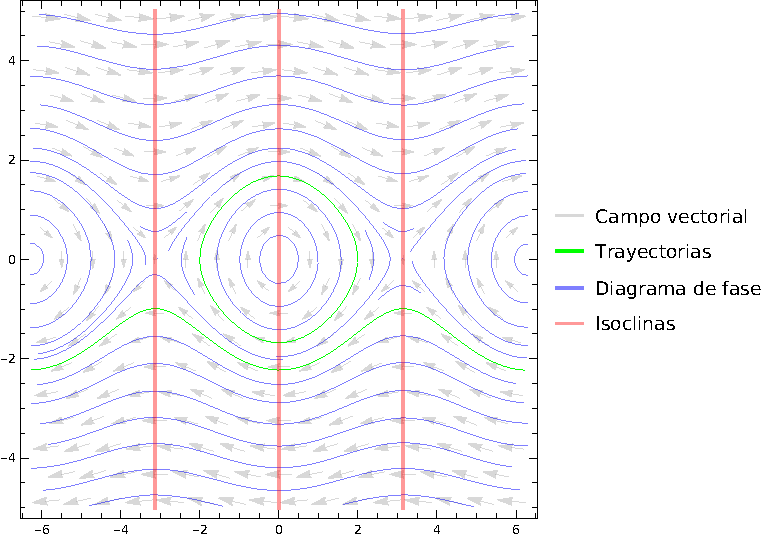
\includegraphics[width=0.7\textwidth]{img/Example.pdf}
	\caption{Ejemplo de campo vectorial, trayectorias, retrato fase e isoclinas ($c=0$) del sistema \eqref{eq: pvi} asociado a $f(x)=(x_{1},\sin{x_{2}})$.}
	\label{fig: example}
\end{figure}

\begin{defi}
	Sea $\mathcal{M}_{n}(\R)$ el conjunto de matrices cuadradas de tamaño $n$ con entradas en $\R$ y sea $A \in \mathcal{M}_{n}(\R)$. Un escalar $\lambda \in \R$ es un valor propio de $A$ si existe un vector no nulo $v \in \Rn$ tal que, $Av = \lambda v$. Un vector $v \in \Rn$ tal que $Av = \lambda v$ es llamado un vector propio de $A$ asociado al valor propio $\lambda$.
\end{defi}

\begin{defi}
	Sea $A \in \mathcal{M}_{n}(\R)$ decimos que $A$ es diagonalizable si existe una matriz invertible $P \in \mathcal{M}_{n}(\R)$ y una matriz diagonal $D$ tal que $P^{-1}AP = D$.
\end{defi}

\begin{defi}
	Un punto $x_{0} \in \Rn$ es llamado un punto de equilibrio o punto crítico de \eqref{eq: sisAut} si $f(x_{0})=0$. Un punto crítico $x_{0}$ es llamado un punto de equilibrio hiperbólico de \eqref{eq: sisAut} si ninguno de los valores propios de la matriz jacobiana $Df(x_{0})$ tiene parte real cero. El sistema lineal \eqref{eq: sisLinAuto} con la matriz $A = Df(x_{0})$ es llamado la linealización de \eqref{eq: sisAut} en el punto $x_{0}$.
\end{defi}

\begin{defi}
	Un punto $x_{0} \in \Rn$ es llamado un sumidero si todos los valores propios de la matriz jacobiana $Df(x_{0})$ tienen parte real negativa; es llamado una fuente si todos los valores propios de la matriz $Df(x_{0})$ tienen parte real positiva; y es llamado un punto silla si es un punto de equilibrio hiperbólico y $Df(x_{0})$ tiene al menos un valor propio con parte real positiva y al menos un valor propio con parte real negativa.
\end{defi}

\begin{figure}
	\centering
	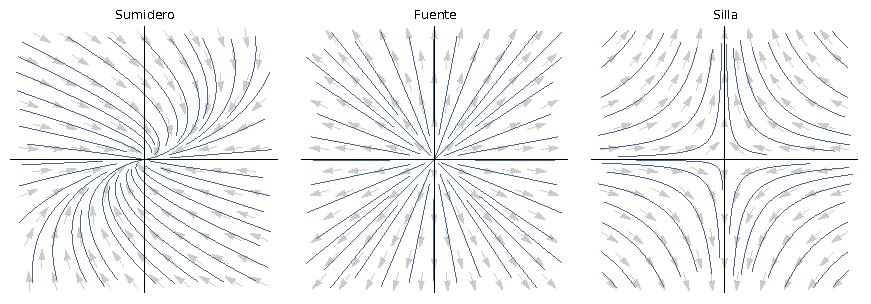
\includegraphics[width=1\textwidth]{img/EquilibriumPoints.pdf}
	\caption{Ejemplo de puntos de equilibrio en el origen de un sistema lineal bidimensional.}
	\label{fig: EquilibriumPoints}
\end{figure}

\begin{teo}[Hartman-Grobman]\label{teo: hartman}
	Sea $E$ un subconjunto abierto de $\Rn$ que contiene al origen, sea $f \in C^{1}(E)$, y sea $\phi_{t}$ el flujo del sistema no lineal \eqref{eq: sisAut}. Suponga que $0$ es un punto de equilibrio hiperbólico. Entonces existe un homeomorfismo $H$ de un conjunto abierto $U$ que contiene al origen hacia un conjunto abierto $V$ que contiene al origen, tal que para cada $x_{0} \in U$, existe un intervalo abierto $I_{0} \subset \R$ que contiene al cero, tal que para todo $x_{0} \in U$ y $t \in I_{0}$
	
	\begin{equation}
		H \circ \phi_{t}(x_{0}) = e^{At}H(x_{0});
	\end{equation}
	
	es decir, H mapea trayectorias de \eqref{eq: sisAut} que estan cerca del origen, hacia trayectorias de \eqref{eq: sisLinAuto} cerca al origen preservando la parametrización por tiempo.
\end{teo}

Si
\begin{equation}
	\dot{x} = f_{\mu}(x) \quad x \in \Rn, \quad \mu \in \R^{k}
	\label{eq: sisParametro}
\end{equation}
es un sistema de ecuaciones diferenciales que depende del parámetro $k$-dimensional $\mu$, entonces los puntos de equilibrio de \eqref{eq: sisParametro} son dados por las soluciones de la ecuación $f_{\mu}(x) = 0$. Cuando $\mu$ varia, el teorema de la función implícita implica que estos puntos son descritos por funciones suaves de $\mu$ que estan lejos de aquellos puntos en los que la matriz jacobiana $Df_{\mu}(x)$ tiene un valor propio cero. El gráfico de cada una de estas funciones es una \textit{rama de equilibrio} de \eqref{eq: sisParametro}. En un punto de equilibrio $(x_{0}, \mu_{0})$ donde $Df_{\mu_{0}}(x_{0})$ tiene un valor propio cero, varias ramas de equilibrio pueden converger, y se dice que $(x_{0}, \mu_{0})$ es un \textit{punto de bifurcación}.

Un \textit{diagrama de bifurcación} de un sistema de la forma \eqref{eq: sisParametro} es el conjunto de todas las ramas de equilibrio mostradas en el espacio $(x, \mu)$.